
\begin{block}{Markov Decision Process (MDP)}
\vspace{0.15cm}
    \begin{center}
    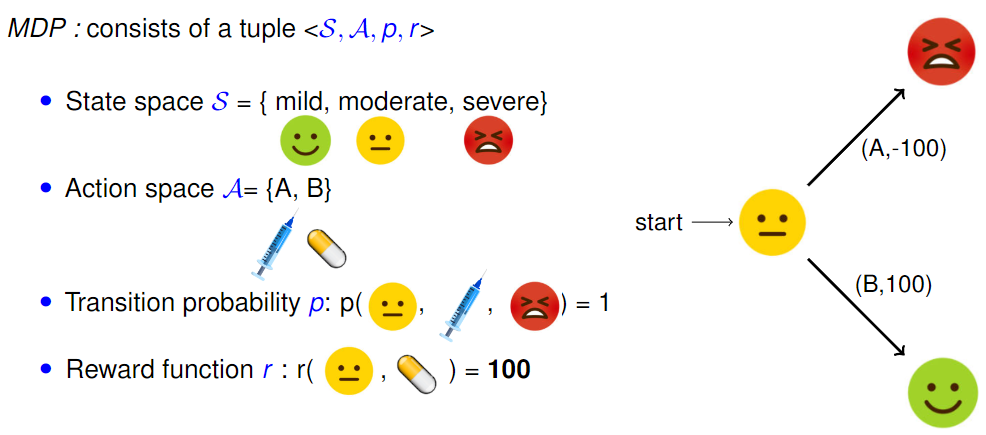
\includegraphics[width=0.95\linewidth]{fig/mdp.png}    
  \end{center}
  \vspace{0.15cm}
\end{block}

\begin{block}{\normalsize{Inverse Reinforcement Learning (IRL)}}
  \begin{itemize}
     \item Given a dataset of expert demonstrations and an MDP model without a reward function, IRL aims to learn a policy $\pi$ 
       from a dataset of expert demonstrations $D_e = \{ s_i, a_i, r_i \}_{i=0}^{N}$.
     \[
       \rho(\pi, r) = \lim_{T \to \infty} \mathbb{E}^{\pi, p_0} \lbrack \sum_{t=0}^{T} \gamma^t r(\tilde{s}_t, \pi(\tilde{s}_t)) \rbrack
     \]
     \item Optimal policy $\pi^* $
     \[
       \pi^* = \argmin_{\pi \in \Pi} \max_{\pi_e \in \Pi} \max_{r \in \mathcal{R}} \rho(\pi_e, r) - \rho(\pi, r)
     \]
    
\end{itemize}
\end{block}






%%% Local Variables: 
%%% mode: latex
%%% TeX-master: "main"
%%% End: 
